\subsection{Lake-at-Rest Over an Uncertain Bed}

This test verifies that well-balanced stochastic Galerkin model preserves the C-property for a lake at rest over an uncertain bed.
An analytic solution of the test preserves the quiescent state forever, but numerical methods that are not well-balanced can produce spurious flows.

To present a challenging test, a rectangular obstacle is introduced to the right of the uncertain hump, so the bed elevation $z$ becomes
\begin{subequations}
\begin{align}
    z(x, a) &= a \sech^2 \left( \frac{\pi x}{\lambda} \right) + \zrectbump(x) \text{,} \\
    \zrectbump(x) &= \begin{cases}
    \amean & \text{if $30 < x \leq 40$,} \\
    0 & \text{otherwise}
    \end{cases}
\end{align}
\end{subequations}

Results of the well-balanced stochastic model are compared with those of a stochastic model having a centred difference approximation of the bed slope source term that is not well-balanced.
The centred difference model is the same as the well-balanced  model except that the stochastic bed slope source term is
\begin{align}
    \Ensemble{\source_i \pcbasis_l} =
    \left[ 0, -g \sum_{p=0}^P \sum_{q=0}^P h_{i,p}
    \frac{z_{i+1,q} - z_{i-1,q}}{2 \Delta x}
    \Ensemble{\pcbasis_p \pcbasis_q \pcbasis_l} \right]^\T
\end{align}

\begin{figure}
\centering
\centering
\begin{subfigure}{\textwidth}
\phantomsubcaption\label{fig:lakeatrest:centred:eta}
\phantomsubcaption\label{fig:lakeatrest:sgm:eta}
\phantomsubcaption\label{fig:lakeatrest:centred:q}
\phantomsubcaption\label{fig:lakeatrest:sgm:q}
\centering
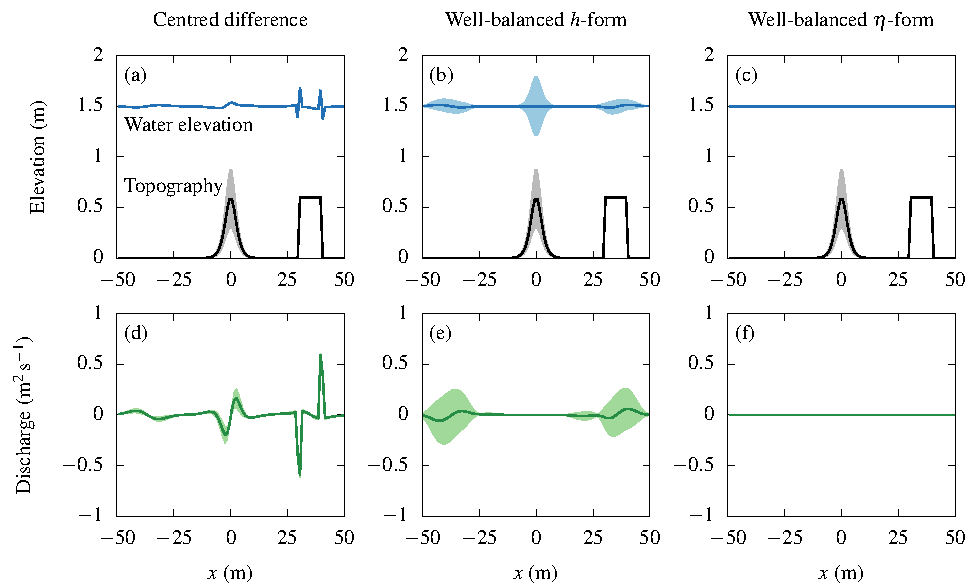
\includegraphics{fig-lakeatrest.pdf}
\end{subfigure}
\caption{Stochastic lake-at-rest solutions at $t = \SI{100}{\second}$.
Mean values are marked by solid lines and shaded regions represent one standard deviation from the mean.}
\label{fig:lakeatrest}
\end{figure}

The test is integrated for \SI{100}{\second} corresponding to about 670 timesteps, and the resulting bed elevation, water elevation and discharge profiles for the centred difference and well-balanced stochastic Galerkin models are shown in figure~\ref{fig:lakeatrest}.
The lack of well-balancing is apparent using the centred difference model: grid-scale standing waves develop at the discontinuities either side of the rectangular hump (figure~\ref{fig:lakeatrest:centred:eta}, \ref{fig:lakeatrest:centred:q}), and a smooth standing wave also develops over the topographic hump.
These errors persist throughout the simulation.
In contrast, the well-balanced stochastic Galerkin model preserves the \cproperty, with discharges accurate to machine precision (figure~\ref{fig:lakeatrest:sgm:q}).

Since the hump amplitude has a Gaussian probability distribution, the tails of the distribution extend to $\pm \infty$.
Hence, there is a non-zero probability that the bed elevation extends above the water level creating a dry region.
The stochastic Galerkin formulation presented here do not accommodate wetting-and-drying processes, and any negative water height will crash the model.
If the stochastic polynomial degree $P$ is increased then the Gauss-Hermite quadrature points in equation~\eqref{eqn:pc-flux} extend further into the tails of the probability distributions, leading to negative water heights being provided as input to the Riemann solver.
Alternatively, if the bed elevation is raised, the water elevation lowered, or the bed elevation uncertainty increased, then negative water heights will also be generated and cause the model to crash.
This is a known problem with stochastic Galerkin methods that use a Weiner-Hermite polynomial chaos expansion \citep{pettersson2014}.

The lake-at-rest test presented in this section confirmed the analytic verification of the stochastic Galerkin \cproperty, with the well-balanced stochastic Galerkin model preserving the \cproperty{} to machine precision.
In the next section, the stochastic model converges on a steady-state flow over an uncertain bed, and the statistics of the flow are compared against a reference Monte Carlo simulation.

%Variance of water elevation, $\sigma_\eta^2$ is
%\begin{align}
%    \sigma_\eta^2 = \sum_{p=1}^P \eta_p^2 \Ensemble{\pcbasis_p^2}
%    = \sum_{p=1}^P \left( h_p + z_p \right)^2 \Ensemble{\pcbasis_p^2}
%\end{align}
